\documentclass[11pt]{article}
\usepackage[margin=0.9in]{geometry}
\usepackage{graphicx}
\usepackage{hyperref}
\usepackage{float}
\usepackage{booktabs}
\usepackage{tabularx}
\usepackage{array}
\usepackage{amsmath}
\usepackage{xcolor}

\hypersetup{colorlinks=true, linkcolor=blue, urlcolor=blue}
\setlength{\parskip}{0.45em}
\setlength{\parindent}{0pt}

\title{Graduation Research Report\\Open-set Fungal Classification and Autoresearch Workflow}
\author{Myco Fungi Project}
\date{April 9, 2026}

\begin{document}
\maketitle

\section{Overview}

This report consolidates the current repository state and converts it into a
practical graduation research plan. The project goal is to improve fungal
species classification from colony images, with special emphasis on the
harder open-set setting: the system should classify known species while also
rejecting previously unseen species.

The repository already contains a strong technical base: a retrieval-based
classification pipeline using Qdrant, finetuned CNN feature extractors,
threshold-based unknown-species detection, autoresearch logs with staircase
visualization, and multiple report artifacts. The next phase is to turn these
separate achievements into one integrated research workflow and one coherent
graduation deliverable.

\section{Problem Statement}

The main graduation target is broader than a standard closed-set classifier.
The project must:

\begin{itemize}
  \item improve open-set classification so unknown fungi can be rejected reliably,
  \item package experiment search into a reusable autoresearch workflow,
  \item provide real-time experiment visualization during runtime,
  \item and deliver a client/server platform for data, metadata, search, and prediction.
\end{itemize}

The core research questions are:

\begin{enumerate}
  \item How can segmentation quality be improved so downstream retrieval is more stable?
  \item Which low-cost backbone gives the best trade-off between quality and deployment cost?
  \item Can an autoresearch loop outperform manual or fixed-grid finetuning search?
  \item How can diverse open-set data be used without damaging closed-set retrieval quality?
\end{enumerate}

\section{Current Baselines}

Table~\ref{tab:baselines} summarizes the most important repo-backed metrics.

\begin{table}[H]
\centering
\small
\begin{tabularx}{\textwidth}{>{\raggedright\arraybackslash}p{4.2cm} >{\raggedright\arraybackslash}X >{\raggedright\arraybackslash}p{4.2cm}}
\toprule
Metric & Current best evidence & Source \\
\midrule
Fixed held-out retrieval accuracy & 83.3\% with EfficientNetB1 finetuned & Final report \\
Alternative finetuned CNNs & 78.6\% with ResNet50 and MobileNetV2 & Final report \\
Best archived 5-fold CV mean & 0.6542 with E1 + weighted(avg) + k=11 & CV archive \\
Historical threshold best & F1 = 0.4587 with \texttt{wtd\_rat\_halving + roc\_opt} & Threshold report \\
Current refreshed threshold baseline & F1 = 0.4000 with \texttt{gnorm\_0\_2\_p\_gnorm\_0\_3 + f1\_grid} & Current threshold log \\
Open-set diverse dataset & 651 images, 45 species, 1,037 segments & Diverse-data EDA report \\
\bottomrule
\end{tabularx}
\caption{Current baselines that define the starting point for the next 6-8 weeks.}
\label{tab:baselines}
\end{table}

Two practical conclusions follow from these baselines. First, finetuned CNNs are
already validated and should remain the primary research direction. Second, the
open-set threshold pipeline is promising but not yet stable, because the current
refreshed baseline is weaker than the earlier documented best.

\section{Dataset Overview}

\subsection{In-domain dataset}

The primary in-domain dataset contains 435 original Petri dish images, which are
processed into 1,305 segmented colony images across 8 \textit{Penicillium} species.
The current fixed evaluation split uses 24 training strains and 7 held-out test strains.

\subsection{Diverse open-set dataset}

The diverse dataset adds broad fungal variation for known-vs-unknown evaluation.
The reorganized version currently contains 651 processed images from 45 species and
1,037 segmented colonies. This dataset is important because it stresses the rejection
behavior of the system instead of only its closed-set ranking accuracy.

\begin{figure}[H]
\centering
\begin{minipage}[t]{0.24\textwidth}
  \centering
  \includegraphics[width=\textwidth,height=4.0cm]{../../../Dataset/full_image/f9036734b8b95250a89d905f01fb67b7.jpg}\\
  \small Processed full-dish image
\end{minipage}
\hfill
\begin{minipage}[t]{0.24\textwidth}
  \centering
  \includegraphics[width=\textwidth,height=4.0cm]{../../../Dataset/segmented_image/f9036734b8b95250a89d905f01fb67b7_0.jpg}\\
  \small In-domain segmented colony
\end{minipage}
\hfill
\begin{minipage}[t]{0.24\textwidth}
  \centering
  \includegraphics[width=\textwidth,height=4.0cm]{../../../Dataset/diverse_data/images/expansum/MEA/T201_ob_30fe3e37_original.jpg}\\
  \small Diverse-data plate image
\end{minipage}
\hfill
\begin{minipage}[t]{0.24\textwidth}
  \centering
  \includegraphics[width=\textwidth,height=4.0cm]{../../../Dataset/diverse_data/images/expansum/MEA/T201_ob_30fe3e37_seg0.jpg}\\
  \small Diverse-data segmented colony
\end{minipage}
\caption{Representative examples from the current datasets used for retrieval and open-set evaluation.}
\label{fig:dataset_examples}
\end{figure}

\section{Current Methodology}

\subsection{Preprocessing and segmentation}

The current preprocessing workflow standardizes plate images before colony-level
retrieval. Heuristic segmentation is already implemented through KMeans and contour
pipelines, and the repository also contains YOLO-format export scaffolding for a future
deep-learning segmentation benchmark.

\begin{figure}[H]
\centering
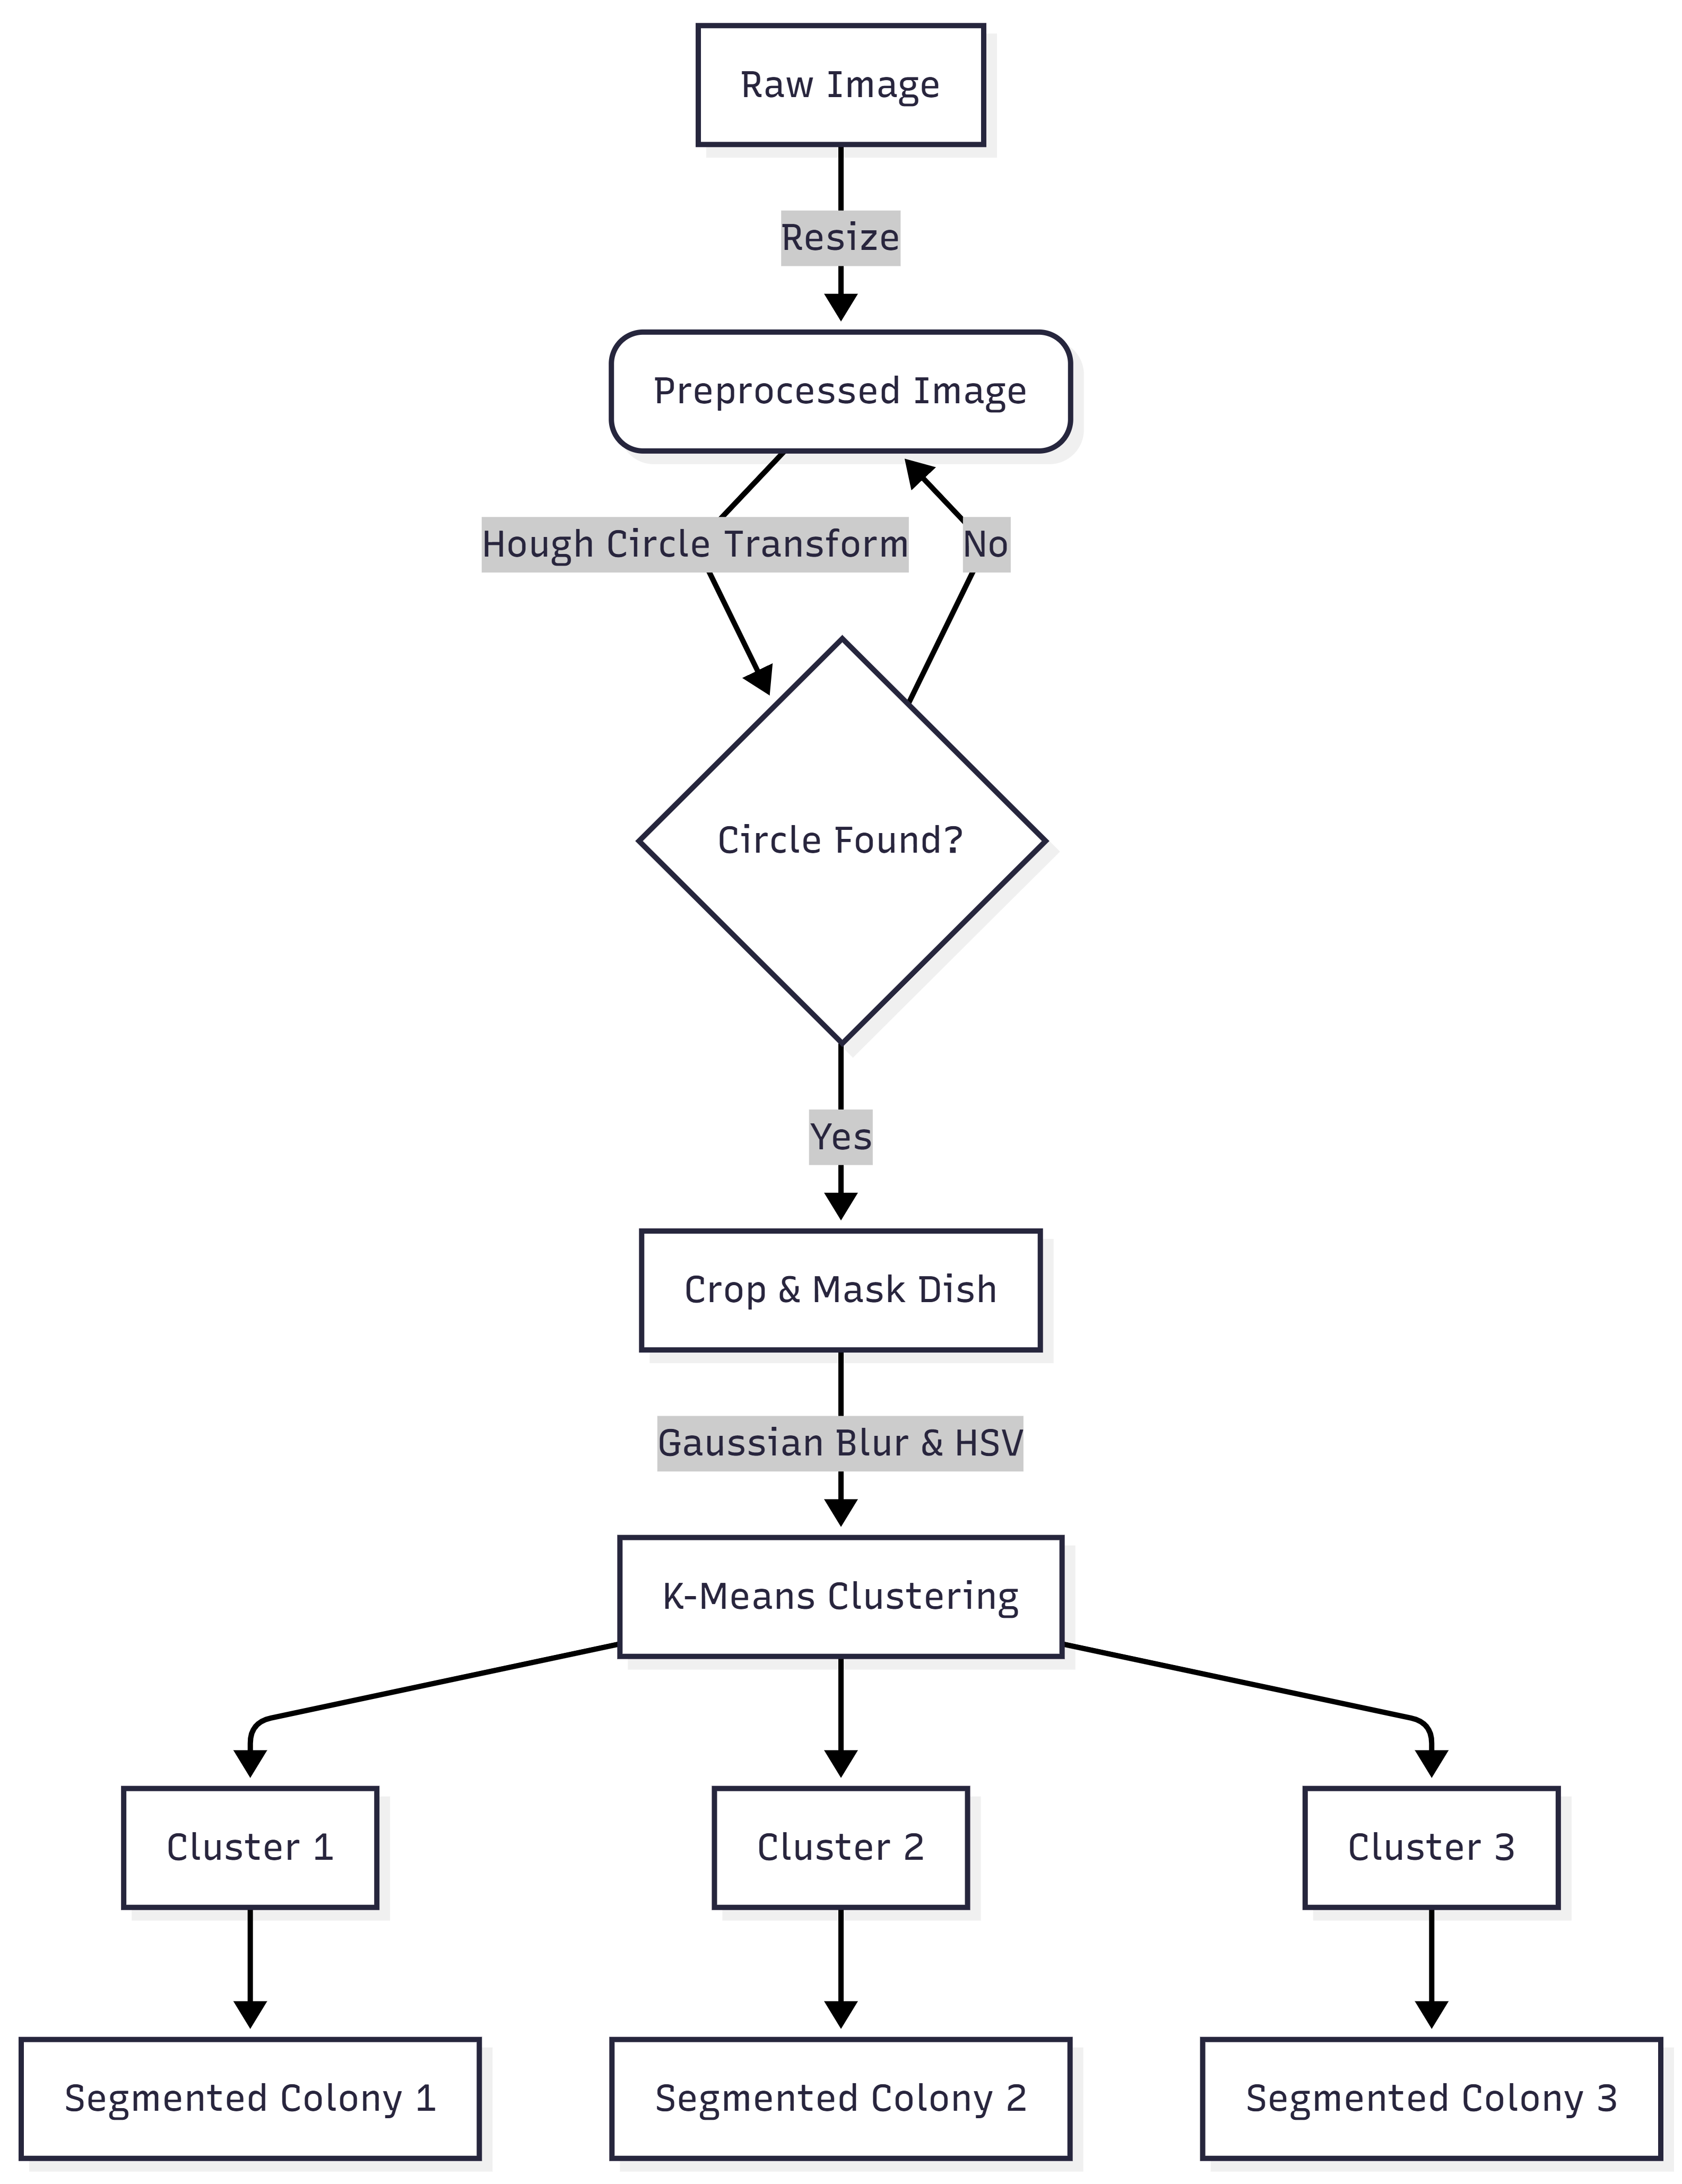
\includegraphics[width=0.92\textwidth]{../../final_gr2/mermaid/preprocessed_diagram_flow.png}
\caption{Existing preprocessing methodology figure showing the image preparation and colony extraction pipeline.}
\label{fig:preprocess_methodology}
\end{figure}

\subsection{Retrieval pipeline}

The main classifier is retrieval-based rather than end-to-end softmax classification.
Each query strain is represented by multiple colony segments. Embeddings are stored in
Qdrant, nearest neighbors are retrieved for each segment, sibling matches are filtered,
and strain-level predictions are aggregated by similarity-weighted voting.

\begin{figure}[H]
\centering
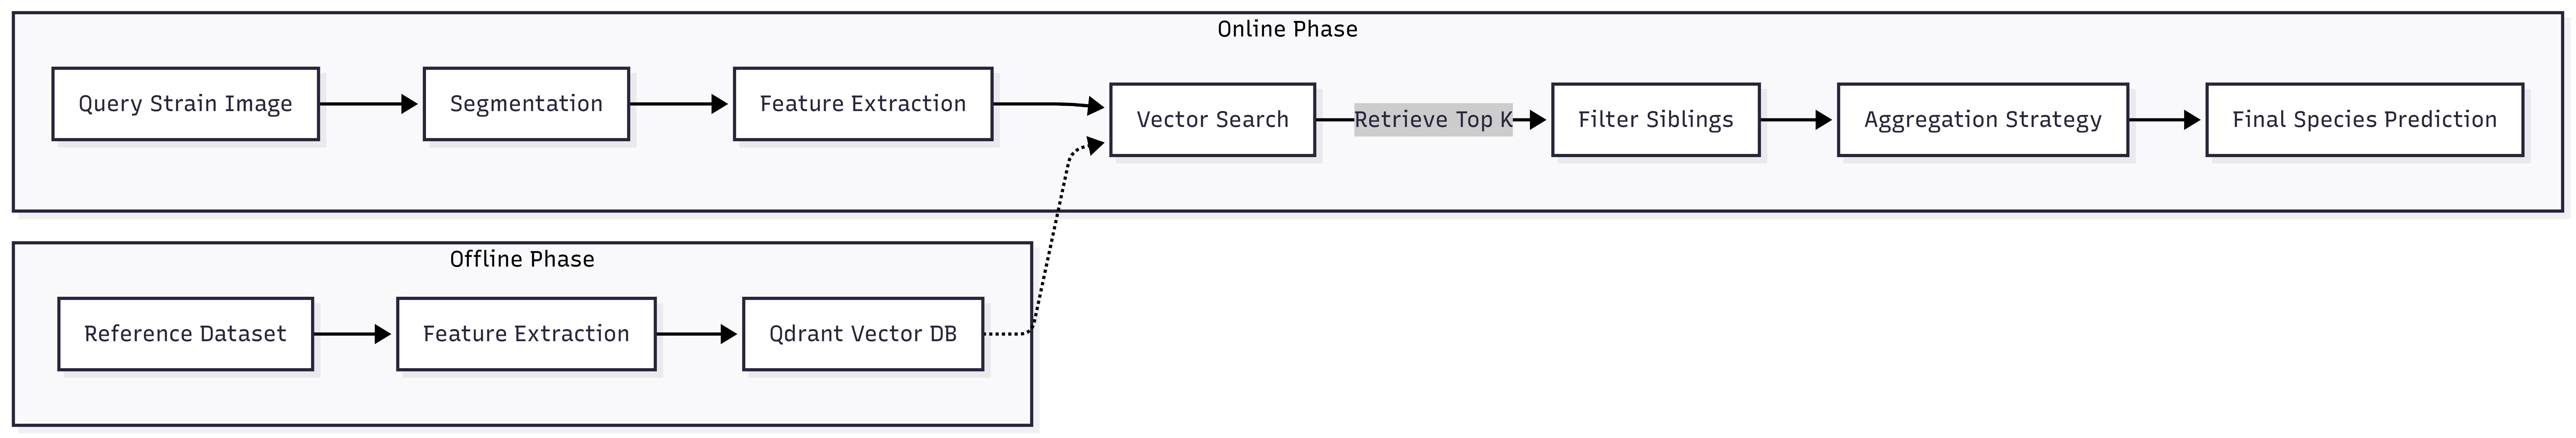
\includegraphics[width=0.92\textwidth]{../../final_gr2/mermaid/query_flow.png}
\caption{Existing retrieval methodology diagram used by the current repository.}
\label{fig:retrieval_methodology}
\end{figure}

\subsection{Autoresearch workflow target}

The next engineering step is to package finetuning into a strict autoresearch loop.
The loop should stay simple. First the research goal and experiment setup are defined.
Then the main agent chooses a method to try. A subagent runs the fixed preparation and
evaluation code, the result is logged, and the main agent uses that new context for the
next iteration. The key design rule is that dataset checks and evaluation stay immutable,
while the editable experiment logic can change loss functions, augmentation, optimizer,
learning rate, and model choice.

\begin{figure}[H]
\centering
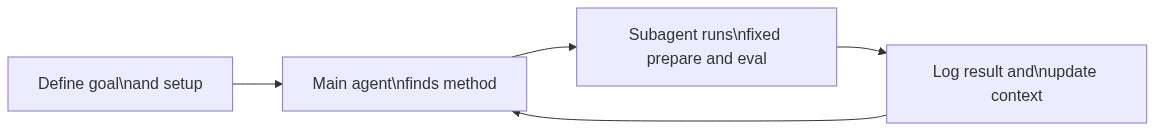
\includegraphics[width=0.58\textwidth]{images/autoresearch_loop.jpg}
\caption{Simplified autoresearch loop. Each trial is logged and then recorded into the staircase-style experiment history defined by \texttt{.claude/rules/experiment-visualization.md}, where every individual experiment becomes one plotted point.}
\label{fig:autoresearch_loop}
\end{figure}

\section{Current Progress and Existing Visualizations}

The project is already beyond the proof-of-concept stage. Retrieval, feature extraction,
threshold search, and dataset reorganization are implemented. The main unfinished work is
to improve open-set robustness, benchmark segmentation properly, and package the workflow
for repeated experimentation and system use.

\begin{figure}[H]
\centering
\begin{minipage}[t]{0.49\textwidth}
  \centering
  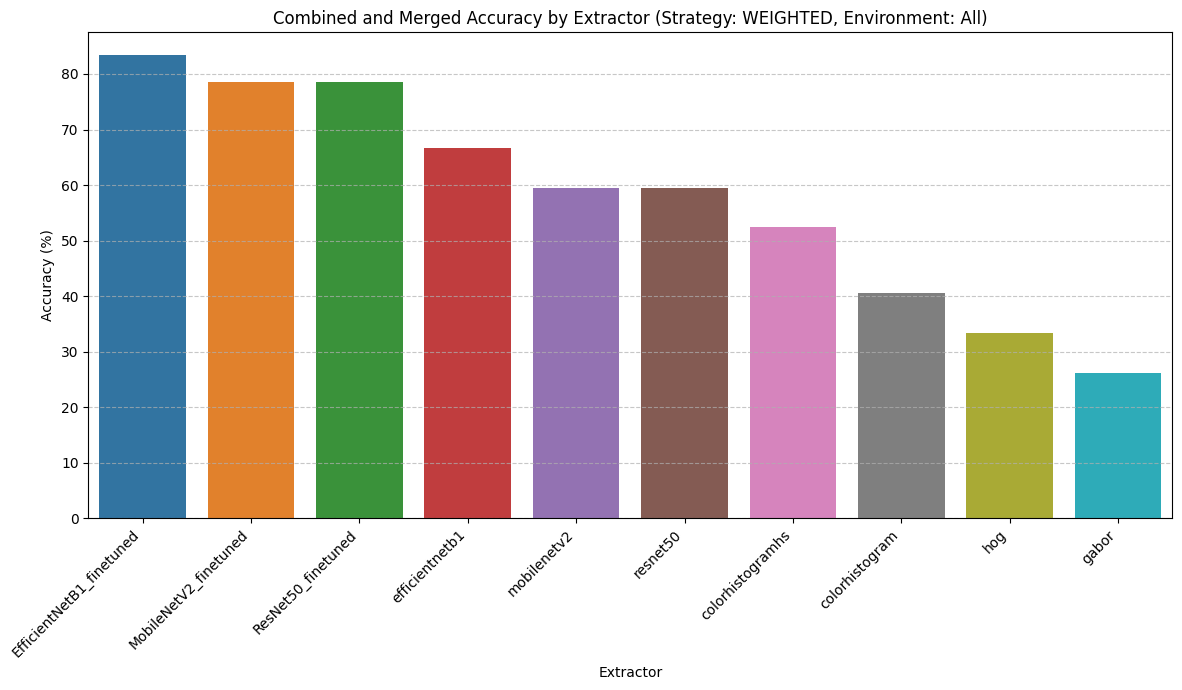
\includegraphics[width=\textwidth,height=6.1cm]{../../final_gr2/training/all_result.png}
\end{minipage}
\hfill
\begin{minipage}[t]{0.49\textwidth}
  \centering
  \includegraphics[width=\textwidth,height=6.1cm]{../../../results/autoresearch/threshold.png}
\end{minipage}
\caption{Existing progress visualizations. Left: closed-set model comparison, where EfficientNetB1 finetuned is currently the strongest fixed-split baseline. Right: threshold staircase showing the history of open-set formula experiments.}
\label{fig:progress_visuals}
\end{figure}

\begin{figure}[H]
\centering
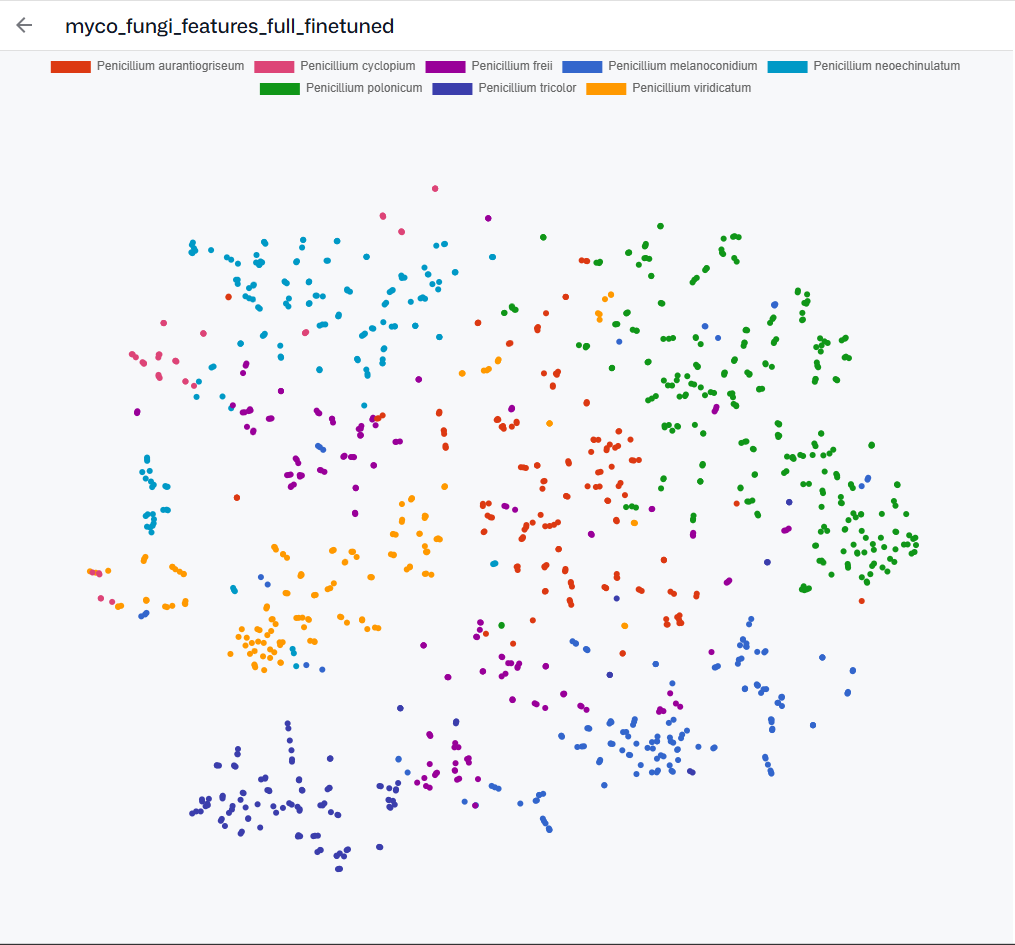
\includegraphics[width=0.82\textwidth]{../../final_gr2/training/images/tsne_finetuned_by_species.png}
\caption{Existing t-SNE visualization of the finetuned feature space. Species-level structure is visible, but overlap remains for difficult pairs, which motivates continued work on embeddings and data quality.}
\label{fig:tsne_species}
\end{figure}

\section{Execution Timeline}

The deadline is June 30, so the realistic implementation window is 6-8 weeks. The
recommended plan uses 8 active weeks and keeps room for revision, advisor feedback,
and demo stabilization.

\begin{table}[H]
\centering
\small
\begin{tabularx}{\textwidth}{>{\raggedright\arraybackslash}p{0.9cm} >{\raggedright\arraybackslash}p{3.5cm} >{\raggedright\arraybackslash}X}
\toprule
Week & Focus & Deliverables \\
\midrule
1 & Freeze scope and baselines & Canonical metric sheet, dataset version lock, requirement questions for Miss Duong \\
2 & Segmentation preparation & Label cleanup plan, annotation subset, benchmark protocol \\
3 & Segmentation comparison & KMeans vs contour vs YOLO/SAM-assisted results \\
4 & Workflow packaging & Canonical finetune experiment path, immutable checks, runtime logging \\
5 & Low-cost finetuning autoresearch & EfficientNetB1 and MobileNetV2 search results and ablations \\
6 & Advanced model exploration & ViT or SimCLR pilot, augmentation study, external-data transfer trial \\
7 & Platform MVP & Upload-search-predict flow, metadata management, experiment dashboard \\
8 & Final benchmark and writing & Final comparison figures, method draft, demo checklist \\
\bottomrule
\end{tabularx}
\caption{Recommended 8-week execution schedule.}
\label{tab:timeline}
\end{table}

\section{Deep-dive Plan}

\subsection{Segmentation improvement}

Current segmentation is still a heuristic baseline. The next step is to create a small
manually verified subset, correct obvious label errors, bootstrap a YOLO-format dataset,
and compare three variants: heuristic segmentation, YOLO-only localization, and YOLO plus
SAM-assisted refinement. The evaluation should measure both annotation quality and
downstream retrieval impact.

\subsection{Finetuning plus autoresearch}

This is the highest-value workstream because the repository already proves that finetuning
substantially improves retrieval quality. EfficientNetB1 should remain the primary research
backbone, while MobileNetV2 serves as the low-cost deployment baseline. A necessary cleanup
task comes first: the finetuning code path is currently split between local scripts and
Colab-oriented scripts, so one canonical experiment package should be defined before the
agent loop is automated.

The main evaluation metric for this workstream should be strain-level cross-validation
retrieval accuracy, because it is a harder and more honest benchmark than the fixed split.

\subsection{Model improvement}

ViT remains a secondary exploration track rather than the main baseline. Existing notes in
the repository already show that ViT is data-hungry on this problem. More realistic medium-cost
improvements are stronger augmentation, hybrid losses such as cross-entropy plus metric learning,
and self-supervised initialization such as SimCLR.

External public datasets should be treated mostly as pretraining or regularization sources,
not as replacements for the in-domain fungal colony data.

\subsection{System platform}

The recommended MVP platform includes:

\begin{itemize}
  \item backend APIs for upload, search, prediction, and metadata CRUD,
  \item a Qdrant-backed retrieval service,
  \item a lightweight metadata store,
  \item a frontend for upload, neighbor inspection, and prediction explanation,
  \item and a small runtime dashboard that reads existing logs and staircase charts.
\end{itemize}

This scope is large enough for a strong graduation demo but small enough to remain realistic.

\section{Questions to Confirm with Miss Duong}

The platform and workflow scope should be confirmed with the advisor early. The most important
questions are:

\begin{enumerate}
  \item Who are the primary users: researcher, technician, manager, or collaborator?
  \item What metadata fields are mandatory when uploading a new sample?
  \item Should predictions be reviewed by a human before permanent storage?
  \item Is unknown-species rejection required in the user interface or only in research evaluation?
  \item Are authentication and user roles required for the graduation demo, or only for future deployment?
  \item Does the system need to connect to external databases or APIs?
\end{enumerate}

\section{Risks and Scope Control}

The biggest risks are annotation time, result-version drift, and system scope creep.
If the project must fit closer to 6 weeks, the must-have items are: one deep-learning
segmentation baseline, one packaged finetuning autoresearch workflow, one refreshed
closed-set and open-set benchmark, and one small client/server MVP. ViT, advanced
authentication, multimodal metadata fusion, and external integrations should be treated
as stretch goals.

\section{Conclusion}

The repository already demonstrates meaningful progress in retrieval, finetuning,
thresholding, and data preparation. The best strategy now is not to restart from zero
with a new model family. The most practical order is: lock the current metrics and dataset
versions, improve segmentation quality, package finetuning into autoresearch, improve open-set
behavior, and then wrap the retrieval core inside a usable client/server demo.

That path fits the 6-8 week graduation timeline and stays aligned with what the current
repository has already proven.

\end{document}
